%% 
%% Copyright 2019-2021 Elsevier Ltd
%% 
%% This file is part of the 'CAS Bundle'.
%% --------------------------------------
%% 
%% It may be distributed under the conditions of the LaTeX Project Public
%% License, either version 1.2 of this license or (at your option) any
%% later version.  The latest version of this license is in
%%    http://www.latex-project.org/lppl.txt
%% and version 1.2 or later is part of all distributions of LaTeX
%% version 1999/12/01 or later.
%% 
%% The list of all files belonging to the 'CAS Bundle' is
%% given in the file `manifest.txt'.
%% 
%% Template article for cas-dc documentclass for 
%% double column output.

% double or single columns
%\documentclass[a4paper,fleqn,longmktitle]{cas-dc}
\documentclass[a4paper,fleqn]{cas-sc}


% If the frontmatter runs over more than one page
% use the longmktitle option.

%\documentclass[a4paper,fleqn,longmktitle]{cas-dc}

\usepackage[numbers]{natbib}
%\usepackage[authoryear]{natbib}
%\usepackage[authoryear,longnamesfirst]{natbib}

% My packages
\usepackage[center]{caption}
\usepackage{multirow}
\usepackage{xurl} % allow arbitrary line breaks in URL strings
\usepackage{xcolor}
\usepackage{soul}

%%%Author macros
\def\tsc#1{\csdef{#1}{\textsc{\lowercase{#1}}\xspace}}
\tsc{WGM}
\tsc{QE}
%%%

% Uncomment and use as if needed
%\newtheorem{theorem}{Theorem}
%\newtheorem{lemma}[theorem]{Lemma}
%\newdefinition{rmk}{Remark}
%\newproof{pf}{Proof}
%\newproof{pot}{Proof of Theorem \ref{thm}}

\begin{document}
\let\WriteBookmarks\relax
\def\floatpagepagefraction{1}
\def\textpagefraction{.001}

% Short title
\shorttitle{Technologies for DMT in ASD users (2017 -- 2022)}    

% Short author
\shortauthors{Removed for blind review} 

% Main title of the paper
\title[mode = title]{How Technology Augments Dance Movement Therapy for Autism Spectrum Disorder: a Systematic Review for 2017 -- 2022}


\author[]{Removed for blind review}            

\begin{abstract}
Autism Spectrum Disorder (ASD) is a neurodevelopmental disorder, characterised by deficits of social communication and social interaction, along with restricted and repetitive patterns in behaviours, activities and interests. People diagnosed with ASD may need lifetime treatment for social inclusion and control of stereotypical behaviour, on which art therapy has played an important role.
Dance Movement Therapy (DMT) has been applied with technology for interventions in social and motor rehabilitation. It has helped people with ASD to integrate in society and develop motor skills, though there are few studies that focus on their artistic expression through the dance and free movements.
This review spans the interventions of DMT in technology for people with autism and other neurodevelopmental disorders, during the last six years, with a query on the technologies and application cases. The purpose of this study is to review more than 50 studies and discuss the most relevant technological aspects classified according to the application theme.
Our general contribution is to give an overview of the current state of the art and provide guidelines for future research on DMT applications for people with ASD, orientated in the development of technologies that combine dance and visual arts for therapy uses.
\hl{This research highlights how technology can enhance DMT by creating immersive and interactive environments that facilitate better engagement and expression for individuals with ASD. The study emphasizes the importance of multidisciplinary approaches, involving artists, designers, and therapists, to develop richer, more inclusive therapeutic experiences. The findings suggest that technology does not need to be advanced or expensive to be effective; simplicity and user-friendliness are key to successful interventions.}
\end{abstract}

% Corresponding author text
\cortext[1]{Removed for blind review}

% Footnote text
\fntext[1]{}

% Keywords
% Each keyword is seperated by \sep
\begin{keywords}
%% keywords here, in the form: keyword \sep keyword
Autism Spectrum Disorder \sep Dance Movement Therapy \sep Interactive Art \sep Embodied Interfaces
\end{keywords}

\maketitle
% INTRODUCTION
\section{Introduction} 
\label{sec1:intro}
Autism Spectrum Disorder (ASD) is an umbrella term for a range of social and communication \hl{issues}, along with \hl{restricted} and repetitive behaviours, detected in early development stages \cite{Lord20}. Children diagnosed with ASD struggle with social integration, \hl{performance of} daily activities, and emotional regulation \cite{Lord18} {and currently have a prevalence of 1 over 100 children} \cite{Zeidan22} around the world. The Diagnostic and Statistical Manual of Mental Disorders (DSM-5) describes core symptoms such as deficits in language or motor development and classifies them in subtypes depending on their social and learning capabilities \cite{DSM-5}. People with ASD find it hard to integrate socially, especially at a very young age, so treatment is primarily focused on children, although it may extend \hl{throughout} a lifetime \cite{Lord20}. 

Compared to typically developed (TD) children, ASD peers perceive \hl{issues} in motor skills and gestural communication. As part of stereotypical behaviour, this can be expressed in involuntary movements, limited joint activity, repeated gestures, and deficits in attention. This implies a lower participation with their peers, reflected at home, school, and in general environments \cite{Oliveira21}.

To overcome these developmental barriers, ASD therapy covers a variety of social and motor skills, specific to the diagnosis of each child. Clinical interventions extend into art practice, which \hl{has} positive outcomes in neurodevelopmental disorders therapy, related to improvements in participation, autonomy communication, and creativity \cite{Ortuño22}. Art therapy can also be applied in its embodied form through dance and free body movements. Dance Movement Therapy (DMT) is an evidence-based practice that utilises movement and dance to promote emotional, cognitive, physical, and social integration of individuals \cite{Crooks2021}.

Dance movement therapy is a space for non-verbal expression and liberty of movement. Therapists see this intervention as a novel standard for self-exploration, autonomy, and movement control.  Dance Movement Psychotherapy (DMP) has the potential to promote various aspects of well-being in children with ASD, as well as reduce self-stimulatory and stereotypical behaviours  \cite{Aithal2021} . For children with ASD and their families this gives them a space for creative development and reduction in stereotypical behaviour \cite{Ziadat22}.

In this scenario, Information Communication Technologies (ICTs) play a mediator role in augmenting DMT interventions. For instance, the use of body sensors helps in data collection of movements and overall interactions, and virtual scenarios are more attractive for gamified interventions. The contexts of application are varied, and the literature finds applications in education, motor rehabilitation, and social therapy \cite{Srinivasan2013}.  In this study, we review the main context groups for technological DMT interventions.

During times of rapid growth in technological advances, therapy spaces for users with special needs have benefited with positive outcomes. Innovation is necessary to engage the user for a better participation. Creation is a natural factor in human development and is manifested in technologies in the maker movement and creative coding. However, the pursuit of creativity with interactive tools during dance movement therapy sessions seems to be explored in a limited set of works. There is still much work to be done on inclusion and accessibility scenarios.

Works of DMT that use technology \hl{for} users with ASD often refer to motor therapy treatments to correct some movements or reduce their stereotypical behaviours. This is something that limits their expression and may be a risk factor for creativity in this group. Additionally, people with ASD need ways of expression that differ from verbal communication. Dance can help as part of an art therapy practice to convey more communicative skills. The integration of technologies into DMT therapy sessions not only aids in overcoming traditional barriers to therapy, such as limited access to specialized therapists, but also enhances the precision and personalization of interventions, thereby improving overall therapeutic efficacy \cite{Kientz2013}.


In  this study, we \hl{searched} the most relevant studies along the lines of DMT applications, with a perspective in technologies and contexts of use. We \hl{selected} a short list of works that help to understand creativity in dance interventions, but also other aspects that are worked in DMT, such as coordination and imitation. We present various topics that may serve to other researchers in the field as well as to give an overview of current DMT works.

This study is conceived to give an overview of how technology can be allied with DMT to find creative expression and the development of fundamental skills. 
% The main purpose of this systematic literature review is to review the integration of technology with dance movement therapy, applied in motor skills for people with neurodevelopmental disorders. 
\hl{Our main research questions aim to gather information on the main themes of application for these interventions, how is  body movement instructed and captured by the technologies used in the studies and how is dance and body expression evaluated during DMT interventions designed for users with neurodiversity conditions.}

This paper is a systematic literature review and is structured in the following manner. Section 1 provides a general introduction, Section 2 outlines the current findings on expression and DMT in therapy for people with ASD. Section 3 details the methods, selection, and inclusion process guided by PRISMA \cite{Pagen71}. Section 4 outlines the main results, divided into a general group and a list of the most relevant works. Section 5 discusses the results and answers the main research questions and provides guidelines for future studies. Finally, Section 6 presents the key conclusions of this research.



% BACKGROUND
\section{Background} 
\label{sec2:bg}
% Poeple  with ASD require lifetime treatment and support for daily activities. In this sense, one area to cover is creativity and self expression. We have seen this helps them in many ways. Findings on these therapies, motor affections in children and adults.
People diagnosed with ASD require lifetime treatment and support to adapt \hl{to} their daily activities, \hl{often facilitated} by therapy and use of devices\cite{Lord20}.
 In the digital era, there are numerous efforts to improve quality of life and social integration through therapy interventions mediated by technological solutions. Art therapy can benefit from interactive applications and user-centred software design to evolve into richer possibilities, such as extending into interactive or generative art with powerful graphical results. In this sense, an overview of previous works should provide insight \hl{into} the main opportunities and challenges in this field.


The scope of this study is to explore the use of embodied applications for interactive interventions in therapies related to dance and movement. Therefore, we define the main concepts that are used \hl{throughout} this research.
Dance Movement Therapy (DMT) is an intervention guided by an expert in which body movement plays the leading role. This can be expressed in free body movements, dance, choreography, as well as body coordination, synchrony, gestures, and imitation \cite{Sheets10}.


In the field of Human Computer Interaction (HCI), body movements are the input for embodied interfaces. In this case, \hl{body} movements trigger a reaction that gives feedback to the user who originated it. Embodied interfaces can be found throughout different technological fields and applications. Creativity is a motor for advances in technological applications, where users can push their ideas further than traditional artistic practice methods. New media art is conceived with the use of digital tools in various art applications. In art therapy, this can help introduce new mechanisms to provide an engaging and innovative experience \cite{Papadopoulou2016}.  Dance programs can be adapted to all abilities and stages, in this case, for social interaction and formation outcomes 
\cite{Reinders19}.

% Why this paper?
% We hope to relate DMT with ASD, given its social benefits, and technology can be useful.
% Cite papers of ASD with creativitiy and Dance Movement therapy. Refer to skills and main benefits of complementary interventions. Technology wise, cite  about attacting and engaging factors through tech apps.

Technology-enhanced therapy offers numerous benefits, particularly in the context of DMT for individuals with ASD. One of the primary benefits is the ability to create immersive and interactive environments that can facilitate better engagement and participation from the users. For instance, mixed reality (MR) and virtual reality (VR) technologies can simulate various scenarios that might be difficult to replicate in a traditional therapy setting, providing a rich, engaging platform for social and motor skill development. Additionally, technology can bridge the gap created by geographical and logistical barriers, making therapy more accessible to a broader population through remote and tele-therapy options. This was particularly evident during the COVID-19 pandemic, where remote therapy sessions became a necessity and showed positive outcomes. Furthermore, the integration of gamification elements in therapy sessions can turn therapeutic activities into enjoyable experiences, thereby reducing anxiety and increasing the likelihood of sustained participation and progress \cite{Parsons2011, Zhang2022}.

Works of DMT that use technology \hl{for} users with ASD often refer to motor therapy treatments to correct some movements or reduce their stereotypical behaviours. This limits their expression and may be a risk factor for creativity in this group. Additionally, people with ASD need ways of expression that differ from verbal communication. Dance can help along as part of an art therapy practice to convey more communicative skills \cite{Takahashi2019}.

Given that\hl{, it} is common for people with ASD to have low communicative skills, they seek different forms of expression and \hl{to} communicate their inner self through their bodies. A creative DMT intervention can have positive outcomes in people with ASD, as it allows them to communicate and connect with their inner self,  reduce anxiety and stress \cite{Martin18}.


% Refer to other studies.
% Trends in Music Therapy have presented other related works, like presented by Ragone. Still, literature is NOT sufficient in terms of DMT interventions, to prodive helpful insights on the areas of work, prevalence and data. Missing guidelines and areas of study.

Currently, DMT has multiple technological applications related to motor and music therapy although not many with dance and expression as the focus of study \cite{Ragone21}. The aim of this review is to gather information about related interventions to provide an overview of this field, in the search of designing future DMT applications for users with ASD.

% This paragraph is correct but should extend to all section. Scope of this study, why is relevant and what we expect to achieve that has not been done.
A study of DMT with technology can help to reveal important aspects of expression and movement solutions for defining future interventions,specially after the global pandemic due to COVID19, tele-dance movement psychotherapy has shown positive outcomes in social development that should be explored \cite{Moo23, Araya2024}. We validate this form of expression, as it brings benefits to children and allows alternative forms of communication and expression.


% METHODS
\section{Methods and materials} %% SECTION 3 %% 2-3 pages
\label{sec3:methods}
This section presents the search strategy and methodology to conduct the systematic literature review. The research questions are presented in \hl{alignment with} the previous sections. This process started with a preliminary search, followed by the main search performed in scientific databases and the selection process.

Aiming to explore DMT interventions mediated by technology in people with ASD and other neurodiverse disorders, we conducted a preliminary search that \hl{yielded} few results. We searched with the keywords: ``autism'', ``ASD'', ``dance therapy'', ``dance psychotherapy'', and ``technology'', and found a literature review of music therapy interventions as well as other \hl{dance movement therapy} projects for people with ASD. Still, the number of articles was not sufficient to conduct a review. 

With the preliminary search, we found that most works used DMT for areas \hl{that involved interdisciplinary projects that extend this type of therapy use}. Most cases treated motor therapy, games, and music therapy with embodied interfaces, though few were defined as dance therapies or related to body expression. \hl{In light of this}, we decided to \hl{conduct} a literature review that includes DMT interventions in all applied areas, and with a special focus on the artistic and expressive side. 

\subsection{Search strategy}
We structured our approach to conduct the literature review in accordance with the Preferred Reporting Items for Systematic Reviews and Meta-Analyses (PRISMA), \cite{Pagen71}. This method provides guidelines to organise this study as a literature review, with a report on the study selection, analysis and discussion of the research findings. This review was conducted following the PRISMA checklist.

First, we use the Goal Question Metric model \cite{Koziolek} to define the purpose and object of study, in this case to perform a literature analysis \hl{of} scholarly papers of technological applications. Our common scheme is to find applications of DMT interventions for users with autism or similar neurodevelopmental disorders, \hl{from the perspective} of software engineering and HCI researchers.

% We define the Goal Question Metric model \cite{Koziolek}, which defines the:
% \begin{description}
%   \item[Purpose] Literature analysis;
%   \item[Object] Scholarly papers of technological applications;
%   \item[Issue] Application of DMT for interventions in autism;
%   \item[Viewpoint] Software engineering and HCI researchers
% \end{description}


The first objective is to characterize the fields of application that have applied \hl{technological} solutions in DMT interventions for ASD users.  The idea is to distinguish in which areas these works are set and understand the scope of their study. We define the first question as:

\begin{description}
  \item[RQ1] \begin{quote}What themes of application has technology contributed in DMT interventions for people diagnosed with ASD?\end{quote}
\end{description}


Second, we need to distinguish which aspects of body movement are observed and evaluated in the DMT interventions for people with ASD. It is also relevant to find what technologies are involved to capture the data and integrate it \hl{into} the applications. Therefore, the second question is:

\begin{description}
  \item[RQ2] \begin{quote} How is body movement instructed, captured and analysed in technological DMT applications for people diagnosed with ASD? \end{quote}
\end{description}


Third, the importance of artistic and self--expression should be noted in DMT interventions, as it is important for social development. We need to find how it is evaluated and managed in the technological solutions implemented for people with ASD. The third question is:

\begin{description}
  \item[RQ3] \begin{quote} How are dance and expression evaluated during technological DMT interventions for people diagnosed with ASD? \end{quote}
\end{description}

We executed the search in the Scopus, ACM Digital Library, Web of Science and IEEE Xplore databases during March of 2023. Based on the preliminary search, the search string was improved. We included ``gestures'', ``pose'', ``body movement'' and got more results. These combined with ``therapy'' and ``psychotherapy'' had a wider range of results. Finally, ``movement therapy'', ``dance therapy'' were added separately \hl{which provided} more results. It is described in table \ref{TABLE:db-search}.


\begin{table}[h]
\centering
\begin{tabular}{p{0.6\textwidth}|p{0.18\textwidth}|p{0.06\textwidth}}
\hline
\textbf{Query string} & \textbf{Database} & \textbf{Results}\\ [0.5ex] 
 \hline
(dance OR movement OR pose) AND (therapy OR psychotherapy OR psychology)&ACM Digital Library & 1833 \\
AND (technology OR application OR app OR software) &&\\
AND (``autistic spectrum disorder'' OR autism OR ``ASD'' OR autistic OR ``neurodevelopmental disorder'') &&\\
\hline
TITLE-ABS-KEY((dance OR movement OR pose) AND (therapy OR psychotherapy OR psychology)) & Scopus & 181\\
AND TITLE-ABS-KEY(technology OR application OR app OR software) &&\\
AND TITLE-ABS-KEY(``autistic spectrum disorder'' OR autism OR ``ASD'' OR autistic OR ``neurodevelopmental disorder'') &&\\ 
\hline
ALL=((dance OR movement OR pose) AND (therapy OR psychotherapy)) & Web of Science & 154\\
AND ALL=(technology OR application OR app OR software) &&\\
AND ALL=(``autistic spectrum disorder'' OR autism OR ``ASD'' OR autistic OR ``neurodevelopmental disorder'') &&\\ 
\hline
((``All Metadata'':dance OR ``All Metadata'':movement OR ``All Metadata'':pose) AND (``All Metadata'':therapy OR ``All Metadata'':psychotherapy OR ``All Metadata'':psychology)) & IEEE Xplore & 46\\
AND (``All Metadata'':technology OR ``All Metadata'':application OR ``All Metadata'':app OR ``All Metadata'':software) &&\\
AND (``All Metadata'':``autistic spectrum disorder'' OR ``All Metadata'':autism OR ``All Metadata'':``ASD'' OR ``All Metadata'':autistic OR ``All Metadata'':``neurodevelopmental disorder'') &&\\
 
\hline
\end{tabular}
\caption{Search queries and results for each database}
\label{TABLE:db-search}
\end{table}

\subsection{Selection of studies}

\begin{figure}
	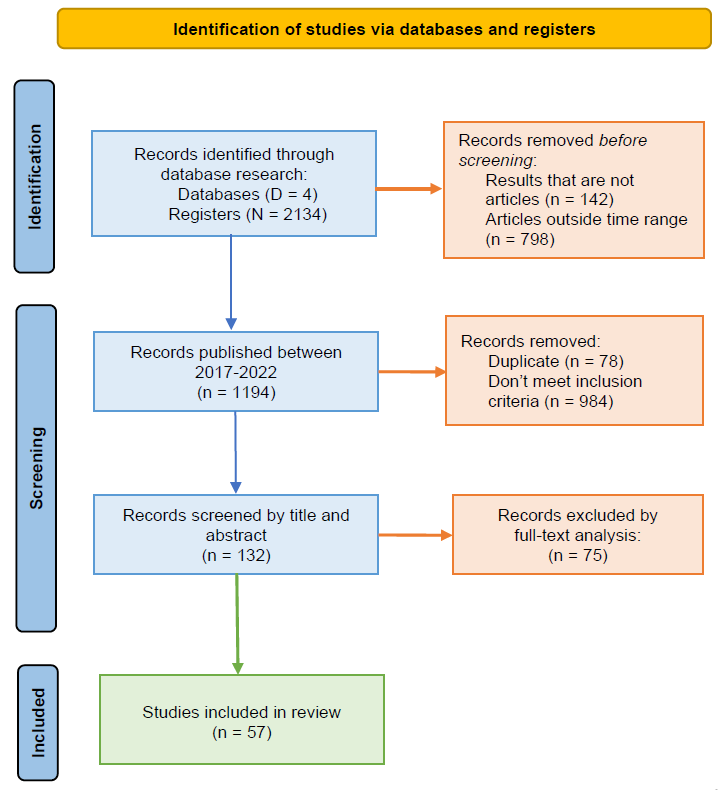
\includegraphics[width=0.65\textwidth]{fig1_search_flow.png}
        \centering
	  \caption{Diagram flow on studies selection}\label{fig1}
        \label{fig:studies-flow}
\end{figure}


The inclusion criteria validate the selection of studies in the research \hl{conducted} along the research community, as well as the topics that \hl{are} relevant to discuss, followed by rigorous selection norms. Selected studies must be peer-reviewed by researchers in the field and written in English, as it is the universal language for scientific publications for most journals and relevant conferences. The studies must be designed for or evaluated ideally with users with ASD, though if the results seem appropriate, designs for similar neurodevelopmental or motor disorders are accepted, in accordance to the other criteria. The projects involved should refer to either an advanced application, demo, prototype, pilot study or design validation of a technology for DMT interventions for the users mentioned earlier. Due to the rapid advancement in technology for emerging contexts, we focus this study \hl{on} the past six years, therefore we consider studies published between 2017 and 2022.


The exclusion criteria help to discard studies that may appear in the database search but \hl{whose} scope of study is not related to the review, or their availability and correspondence \hl{with} the addressed themes. First, we discard all results that were not peer-reviewed articles, i.e., full book referring a proceeding of conference, report., as well as duplicated references. \hl{Also, papers are excluded if they are } not available online or are located in websites that are difficult to access. Studies that involved clinical or medical perspectives such as rehabilitation, limb movement, orthopaedic, or related, and movements such as eye tracking, involuntary movements, and gestures that are used for alternative communication are not considered as they do not reflect DMT objectives. Finally, studies that are literature reviews or do not specify about a single project that can be analysed or evaluated \hl{are also excluded}.


The selection process is described in Fig. \ref{fig:studies-flow}. 
In the identification phase, we obtained a total of 2134 studies from the four databases. First, we discarded 798 articles that were published outside the year range of 2017 and 2022 and 142 that referenced congress proceedings or books titles but had no content. We used Zotero to remove 78 duplicates. In the screening phase, 984 articles were discarded \hl{based on} the inclusion/exclusion criteria. Then, 75 were discarded \hl{after full-text} analysis. 

\subsection{Data collection}
As for Dance Movement Therapy (DMT), we \hl{considered} body movement related to body gestures, facial expressions, limb coordination and rhythm synchrony. Application contexts must be therapy interventions \hl{focused on} the topics of social skills, behaviour, or physical training.

A total of 57 contributions were selected for this study, \hl{involving} body movement-based application \hl{within} the contexts of therapy for ASD and other neurodevelopmental disorders. Of these, only 15 were considered as a full dance movement therapy intervention with an objective of expression or creativity. In this section, we will give an overall view of the studies that met the inclusion criteria and then we will analyse deeply the short list of papers.

For each revised paper, we extracted the themes of application, technology, DMT aspect of study, user range, and number of users.




% RESULTS
\section{Results} 
\label{sec4:results}

This section reports relevant information from all selected studies, based on the classification of all included papers. Projects differed in its own nature and objectives but had similar themes of application that will be described in the following subsection, regarding the use of technology and purpose of the intervention. As a general classification, we seek for a setup, applications, or system of execution with any aspect that requires movement, body actions, or any form of \hl{dance movement therapy}. We have classified the studies according to the technology used, the aspect of DMT to evaluate and testing the user group.

The ensuing part of this section addresses RQ1 by offering a comprehensive overview of our findings, organised according to demographic factors, technology aspects, and the specific domains of study, as elaborated in Sections \ref{sec4:results-dem} and \ref{sec:app-contexts}, respectively. The overview of technology themes that responds to RQ2, is described in Section  \ref{sec:tech-fields}. To respond to RQ3, in Section \ref{sec:4-express}, we highlight a curated selection of studies that delve deeper into the most pertinent contributions within this review. The results gather the necessary information to address the research questions in the following Discussion Section \ref{sec5:discussion}.

\subsection{Demography of results}
\label{sec4:results-dem}
Most studies were designed for a target group of users with a neurodevelopmental disorder, most cases with a special focus on ASD affections. The user group for studies that included evaluation are noted in Figure \ref{fig:user-groups-years}. Children are the predominant group of study, across all ages and developing stages. A total of 44 studies involved children, 36 of them children diagnosed with ASD and 6 with a comparison of ASD with Typical Developing (TD) children, as seen in Figure \ref{fig:user-groups-general}. According to each context, children had different characteristics, though few studies made differences regarding ASD subtypes. Some focused on non-verbal users \cite{McGowan17, Ragone22} , sensory-based affections \cite{MarquezSegura19} and severe autism \cite{Giraud21}.

In evaluation case studies, user participation has an average of 14.31, with a standard deviation of 12.6 and a median of 10 users. Most of the evaluations involved users in the age range of 4 to 12 years, the most frequent groups were 5-10 years old. The participation of caregivers, such as family members or therapists, was conditioned to the scope of the study, although most applications only mention the experience of the children.

\begin{figure}
	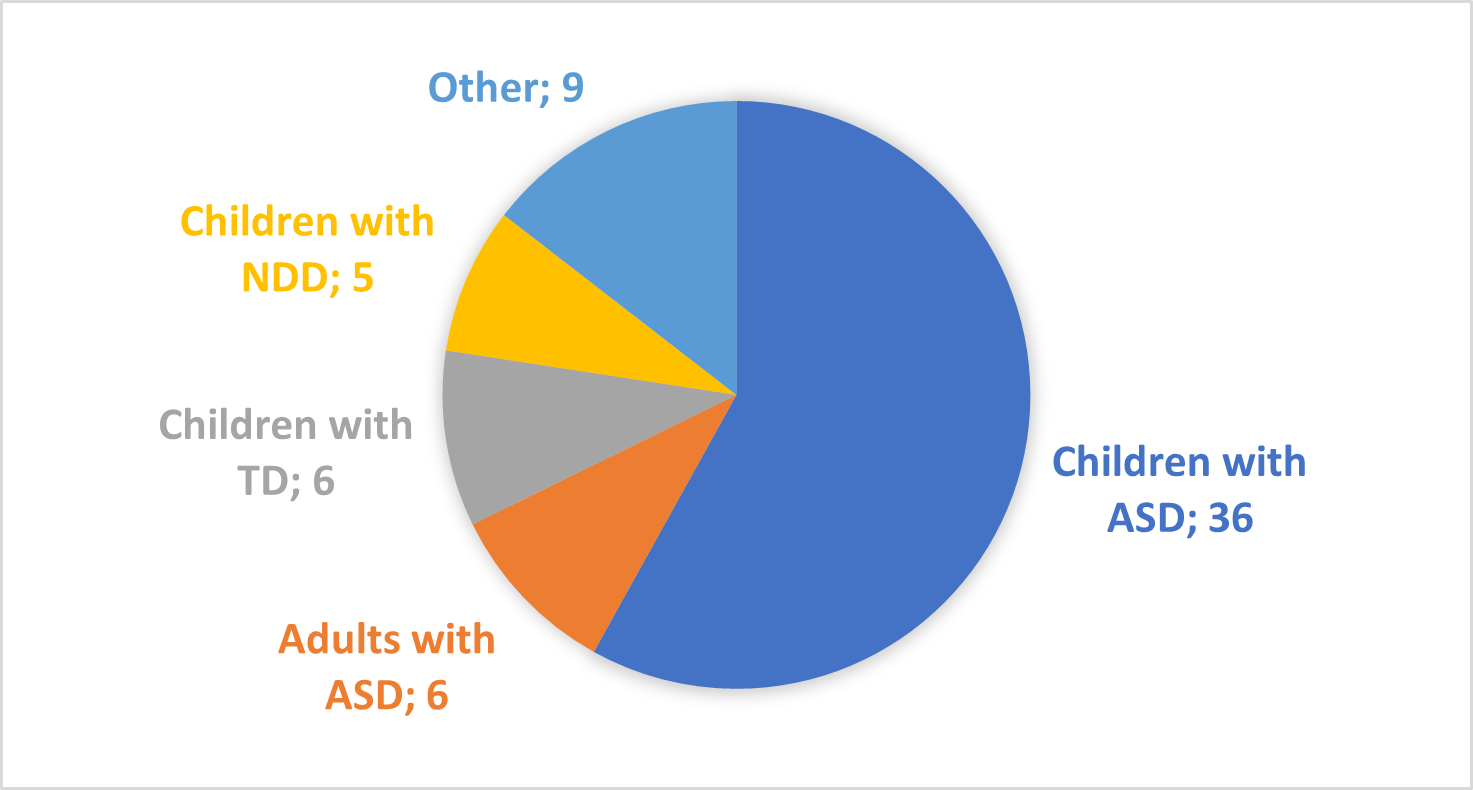
\includegraphics[width=0.65\textwidth]{fig2_user-group-general.png}
        \centering
	  \caption{User groups}
        \label{fig:user-groups-general}
\end{figure}

\begin{figure}
	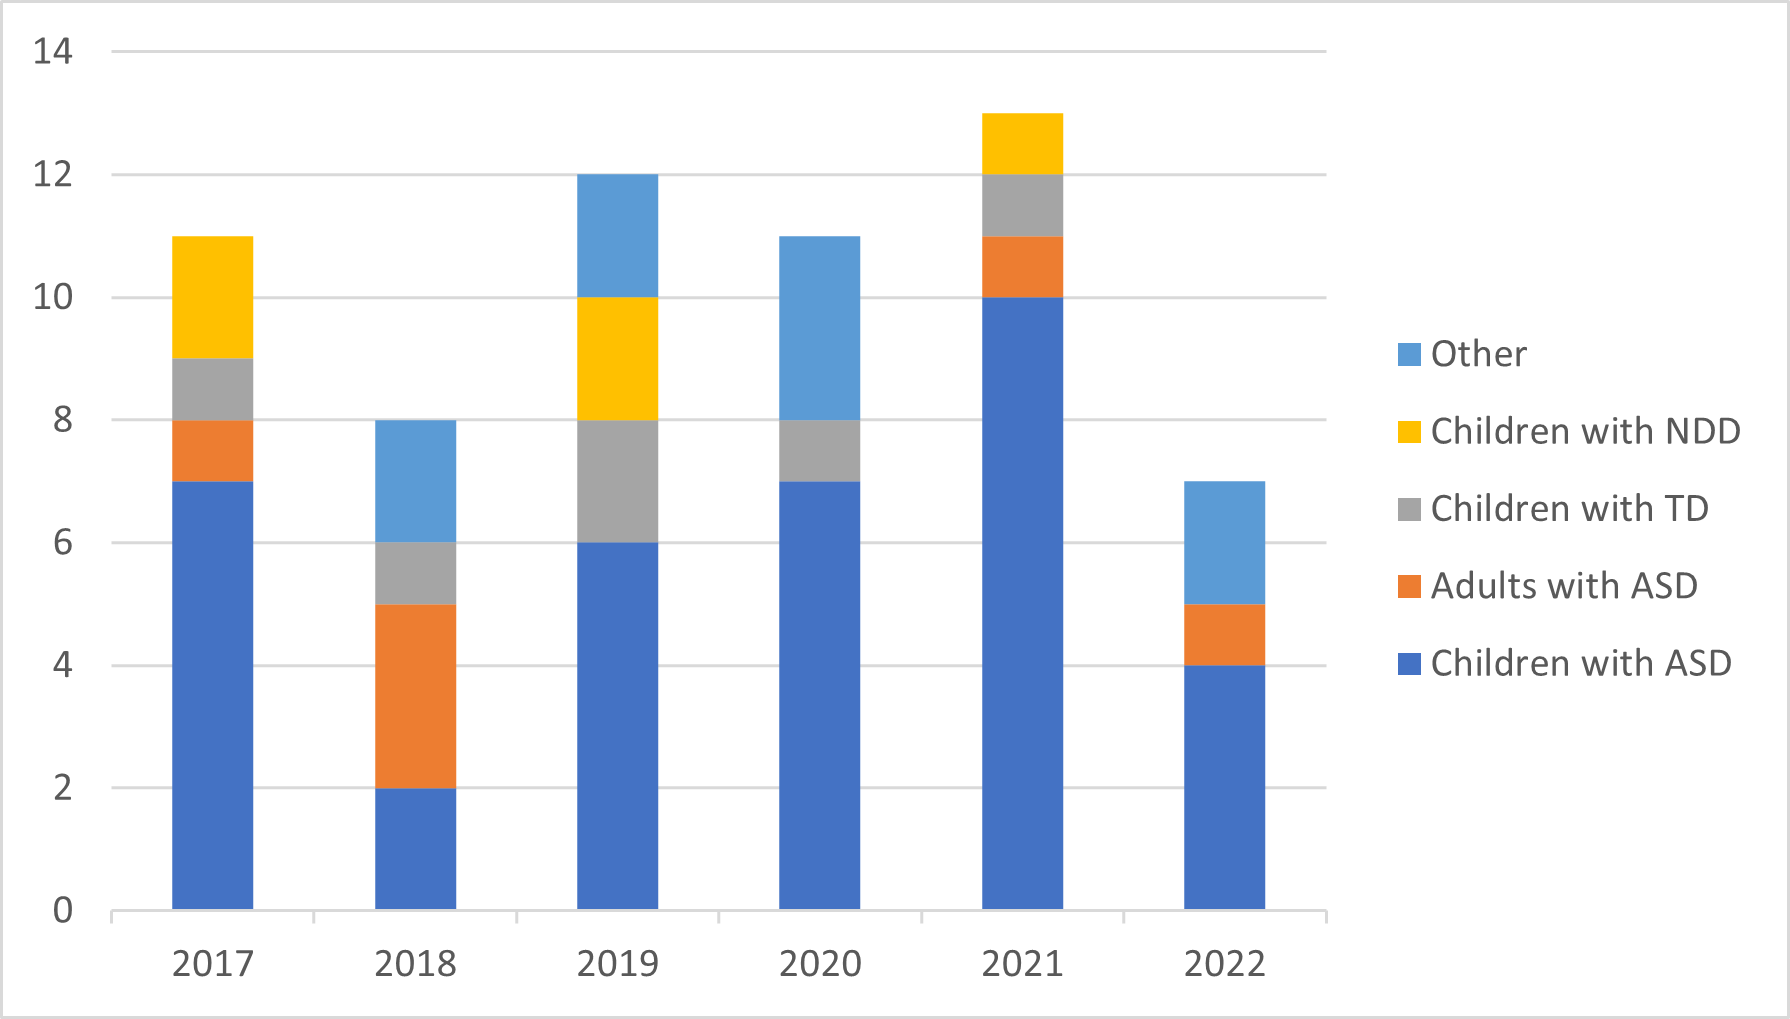
\includegraphics[width=0.65\textwidth]{fig3_user-group-years.png}
        \centering
	  \caption{User groups in evaluation over the years}
        \label{fig:user-groups-years}
\end{figure}

Another relevant aspect to notice is the low number of participants in user evaluations, presented in Figure \ref{fig:user-count-eval}. This number is of 12 or fewer participants in 62.7\% of the reported studies, and only 6 studies have 24 or more users during the evaluation phase. This is explained due to the nature of the participants and their age range may have limitations on finding a larger group. 
As part of the evaluation, research studies involving users with special needs, and children in particular should be approved by ethical committees and follow protocols. Only 12 studies had an explicit declaration, given in most cases from universities and research centres. No further information about ethical implications is mentioned, such as user consentments and data treatment.

\begin{figure}
	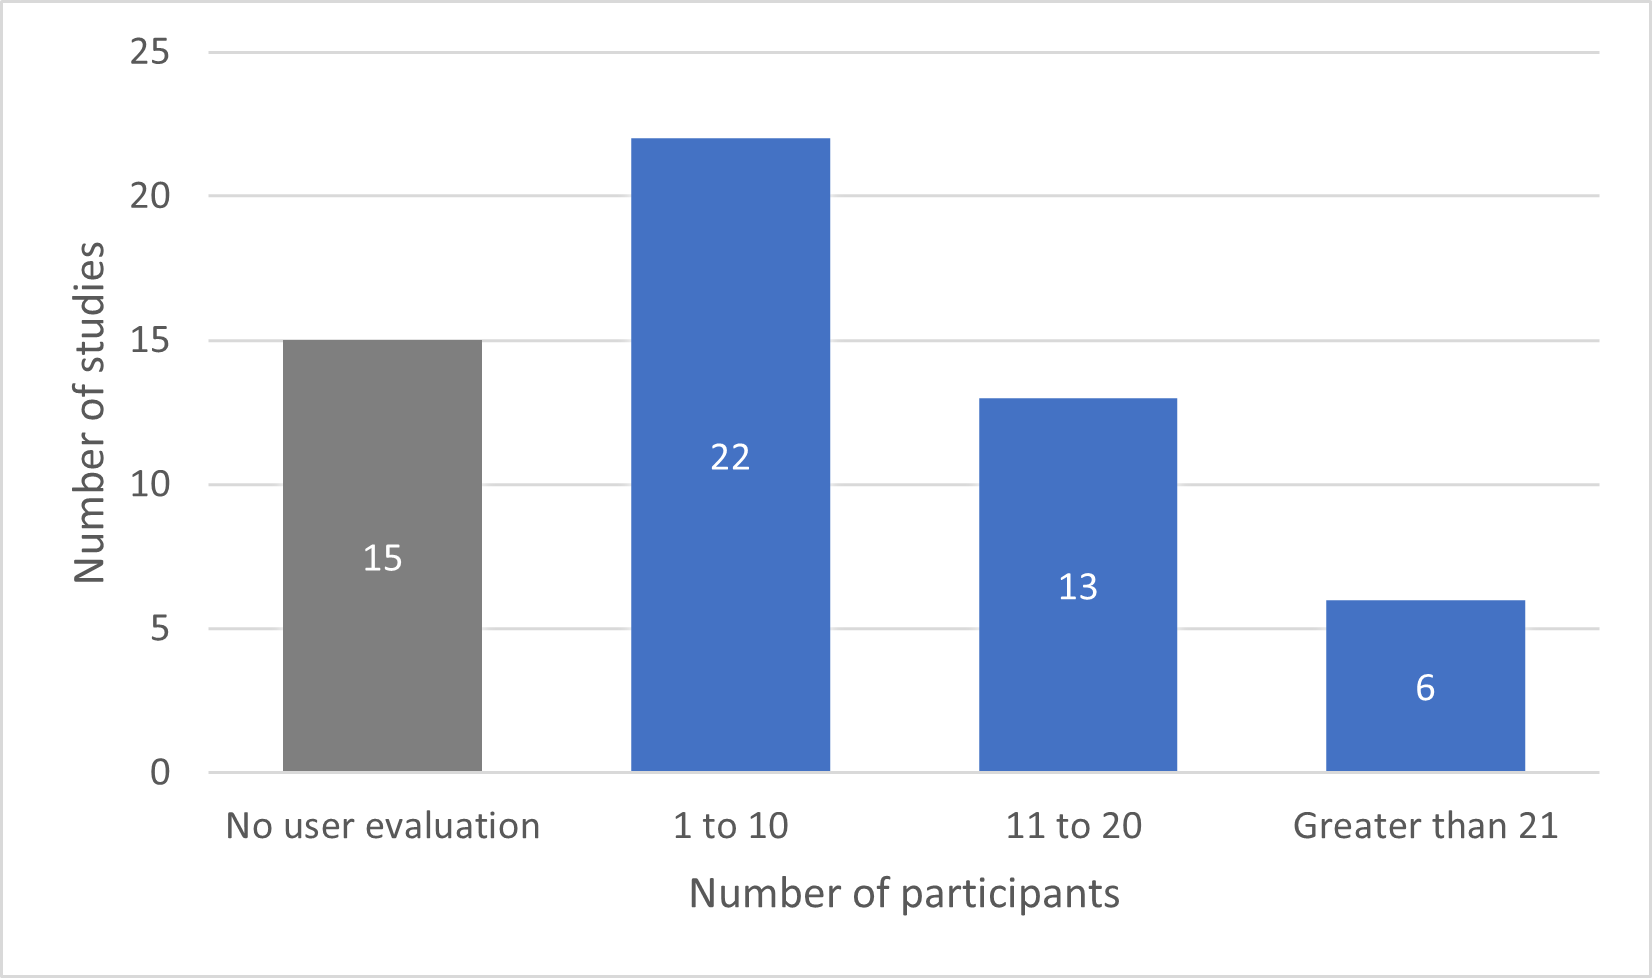
\includegraphics[width=0.65\textwidth]{fig4_user-number-eval.png}
        \centering
	  \caption{Number of participants in evaluations}\label{fig:user-count-eval}
\end{figure}

The specific DMT can include gestures, body balance, synchrony with music, coordination, repetitive movements like hand flapping. Music therapy is related as dance works along rhythms to create a choreography and synchrony. In this case, it is considered if the music helps to produce a body movement with a task. Expression is stimulated by free movements of body self-recognition.

The main types of DMT are reflected in Figure \ref{fig:DMT-types}, noting that coordination is the most frequent, present in a third of the studies. Dance, imitation and gestures are the following research aspects, where balance, exercise and general body movements represent a small group of interventions.

\begin{figure}
	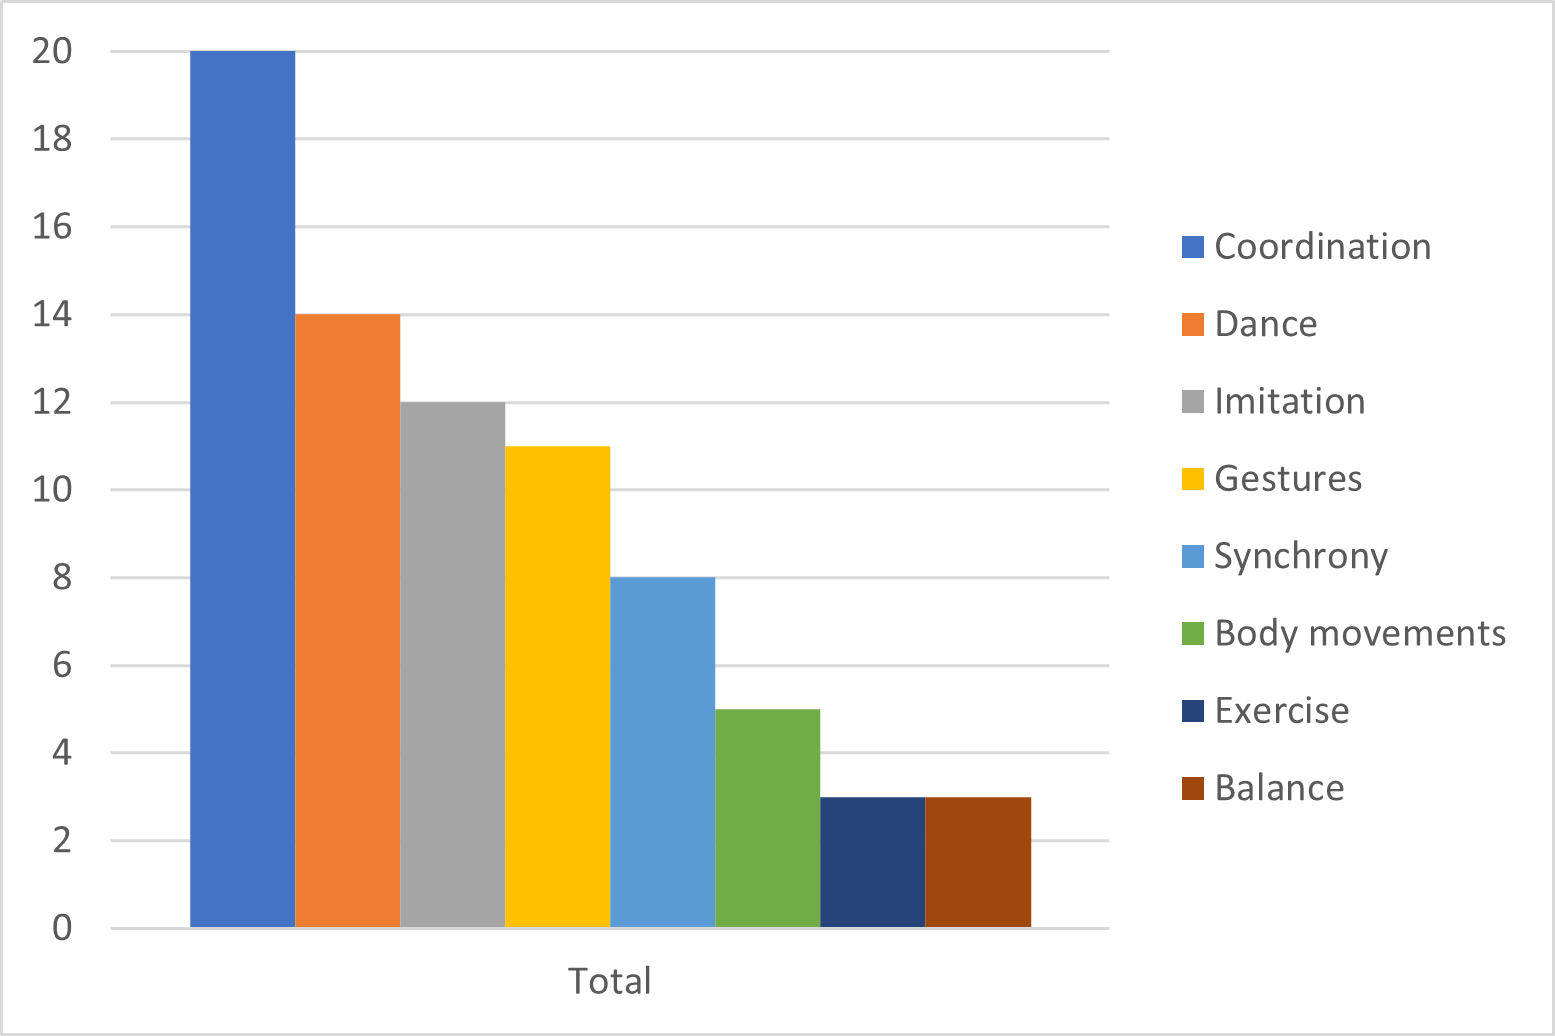
\includegraphics[width=0.65\textwidth]{fig5_DMT-types.png}
        \centering
	  \caption{DMT areas approached in articles}
        \label{fig:DMT-types}
\end{figure}

\subsection{Main application contexts}
\label{sec:app-contexts}
This section presents contributions that keep relation to aspects of DMT in technological interventions across different contexts of applications. Contributions are classified according to their application fields, with the major groups of therapy, games, physical training, and dance.

People with autism or other neurodevelopmental disorders require therapeutic treatment to handle different aspects of their life, so the range of applications is broad and constantly evolving. A total of 47 studies were classified as therapy interventions, mentioned therapeutic scenarios, or included experts related to the field. We classify according to strict therapy interventions in table \ref{TABLE:area-therapy}, motor interventions \ref{TABLE:area-motor} and others \ref{TABLE:area-other}.

One of the major challenges is to develop an effective yet engaging intervention, especially for younger users. The rest of works are classified are part of a training or exercise system, or presented expression with the body or facial expression. A total of 16 works were identified as preliminary or pilot studies, \hl{including four} design validations by experts, that wish to extend in future advanced applications.


\begin{table}[h]
\centering
\begin{tabular*}{6.2in}{p{0.7in}|p{0.85in}|p{0.36in}|p{3.5in}p{0in}}
\hline
Area   & Sub area   & Number & References  &  \\ \hline
\multirow{5}{*}{\centering Therapy}
    & Serious Games Therapy & 14 & \cite{Raygoza-Romero21, DeCarolis21, Simeoli20, Telisheva20,  Rosly20, Martinez-Mones19, Wasserman19, Ruiz-Rodriguez19, Ardalan19, Crowell18, AltizerJr18, Caro18, Sharma18, Castelhano17}
    &  \\\cline{2-4}
    & Music Therapy  & 8 & \cite{Ragone22, Mcgowan21, Ma21, Ragone20, Vargas20, Ragone20OS, Yi-Hsiang18, McGowan17} &  \\
    \cline{2-4} 
    & Dance movement therapy & 4 & \cite{Brown22, Trajkova20, Ringland19, Suzuki17} &  \\
     \cline{1-4}
\end{tabular*}
\caption{Selection of studies involving therapy}
\label{TABLE:area-therapy}
\end{table}

\subsubsection{Therapy}
\label{sec:app-contexts-therapy}
In the context of therapy, serious games offer an engaging and attractive support for the interventions, that helps to strive to an objective through a gamified experience. We have found 14 studies that have games as their main subject, with a range of applications that spans different technologies and environments.

\hl{Socially Assistive Robots (SARs)} for robot-mediated therapy have an engaging aspect, as children interact with a humanoid companion of similar size to guide and replicate actions in the context of game interventions. In these examples, children interact with robotic companions for gesture recognition \cite{DeCarolis21}, automatic engagement recognition \cite{Telisheva20} and tele-rehabilitation \cite{Rosly20}. \hl{Overall, SARs offer a higher engagement level, as noted through video observation} \cite{Telisheva20} \hl{, however further evaluation is needed to imply larger conclusions as user validation  is pending in this stage for selected works.}

Virtual and video games are not only designed for leisure experiences,\hl{these interventions extend their use for social and behavioural skills development,} such as dance as part of inclusion play \cite{Wasserman19}, multisensory stimulation \cite{Castelhano17}, anxiety relief\cite{AltizerJr18} and embodied digital learning \cite{Martinez-Mones19}. \hl{Exergames are games that rely on exercise and movements, to support cognitive and motor skills- in this sense, visual-motor coordination exercises with adults} \cite{Caro18} \hl{and children} \cite{Raygoza-Romero21}, help them to gain more autonomy and motivation. \hl{These tools have been validated by experts through focus groups, custom questionnaires and interviews with experts and families of children with ASD} \cite{AltizerJr18, Crowell18, Caro17}. \hl{The engagement has been assessed with the Technology Acceptance Model (TAM) Questionnaire} \cite{Raygoza-Romero21, Vargas20}, \hl{the Game Experience Questionnaire (GEQ)} \cite{Caro18} \hl{and Test of Playfulness} \cite{Castelhano17}. \hl{Video analysis with the Mechanics Dynamics and Aesthetics (MDA) framework} \cite{Wasserman19} \hl{noted that users need more ways to express themselves and that more dance options should be available in games.}

Music therapy consists of sessions conducted by a therapist with the use of sounds, rhythms, or musical instruments to express an idea \hl{or to promote self-expression, generally with coordination and musical synchrony skills}. Works include movement coordination \cite{Ragone22, Vargas20}, musical composition based on movements \cite{Ragone20OS, Ma21}, interactional synchrony with musical stimuli \cite{Mcgowan21, McGowan17} and tempo synchrony \cite{Yi-Hsiang18}. \hl{In general, music interventions motivate the users to receive audio feedback to their body movements, in an action-reaction format, using tempo and musical synchrony measured with instruments such as a metronome}\cite{Yi-Hsiang18}\hl{. Social interactions are counted as social motor synchrony instances with the Motion Energy Analysis (MEA)} \cite{Ragone22, Ragone20OS} and also as observed by experts in behaviour analysis (ABA) for the number of occurrences of musical and non-musical behaviours \cite{Mcgowan21, McGowan17}. 


\hl{A group of interventions identified solely as dance movement therapy give a larger importance of expression through dance, in our study, only four works were} identified as applications of dance with technology, with joint movement through video calls \cite{Brown22}, ballet dance analytics \cite{Trajkova20}, dance augmentation for remote therapy \cite{Ringland19} and dance with a robot \cite{Suzuki17}. \hl{These works explore dance over remote scenarios, with guidance given by virtual characters for children dance interventions. The evaluations have been made by testing systems at home, interviews with experts} \cite{Ringland19} \hl{and questionnaires over the Social Responsiveness Scale} \cite{Suzuki17}. \hl{Overall the findings, refer that the use of technology is engaging for children with ASD, but may need further research to note long-term impact.}

\begin{table}[h]
\centering
\begin{center}
\begin{tabular*}{6.2in}{p{0.85in}|p{0.82in}|p{0.35in}|p{3.5in}p{0in}}
\hline
Area   & Sub area   & Number & References  &  \\ \hline
\multirow{2}{*}{Physical training}
    & Motor training & 8 & \cite{Soprani22, Hocking22, Cibrian21, Syahputra21, Santos20, Bansode19, Lee18, Cornejo17}  &  \\  \cline{2-4}
    & Training system   & 4   & \cite{Fassina22, Giraud21, Zhao21, Oprea17}  & 
    \\ \cline{2-4}
    & Exercise  & 4   & \cite{Baharin19, MarquezSegura19, Ardalan19, Bittner17}    &  \\\cline{1-4}
\end{tabular*}
\caption{Selection of studies in motor areas}
\label{TABLE:area-motor}
\end{center}
\end{table}

\subsubsection{Motor training}
\label{sec:app-contexts-motor}
As part of healthy habits, promotion of exercise is \hl{crucial for general development. These interventions require an instructor to guide the activities, which can be developed as part of a workshop, class or game.}

Motor therapy consists of the control of specific body limbs and general motor skills development. In neurodiverse population the goal is to reduce stereotypical behaviour and adapt to routine tasks. Some examples of therapy for limb movements include coordination exercises with interactive sonification \cite{Cibrian21}, a game of imitation exercises with a robot guide \cite{Santos20}, a gesture recognition model based on electromyography \cite{Syahputra21} and a virtual environment for motor rehabilitation exercises \cite{Soprani22}.

Special education adapts to children with ASD, as they need to feel motivated during physical activities. This has been done during sessions in a projection \cite{Cornejo17} and virtual \cite{Hocking22} reality environments.
Social aspects can be worked by result of the body therapy, such as collaboration with peers, joint tasks and enhance communication skills.


Some skills need to be trained well enough to be fully developed, in this case, with the development of a training system. Solutions involve gesture training in robot-therapy \cite{Fassina22}, joint coordination tasks with a tangible object \cite{Giraud21}, haptic devices for hand movements and grip control \cite{Zhao21}, and a gesture recognition classifier \cite{Oprea17}.

Physical activities are given by interventions that use body movements for exercise and training.
An interactive circle dance game for children for movement synchrony with movement captured by an Arduino board, sensors and LED lights \cite{Baharin19}. Children had to dance in groups with a colour object that provided visual feedback, according to the group movement coordination. The girls group proved to be more coordinated than the boys group, larger mixed groups took less time to complete game.

\subsubsection{Expressiveness and behaviour studies}
\label{sec:app-expression}
\hl{A group of studies that involved the expressiveness and behaviour patterns of children with ASD through a diversity of applications involving body movement and interaction. Self-expression has been explored with a tangible object} \cite{Wilson20}\hl{, wearable motor sensors} \cite{Giomi18}\hl{, also mixed reality has been used for LEGO objects interventions} \cite{Sayis21} \hl{and mobile AR filters for gestural expression} \cite{Pohl20}.

\hl{As noted in most studies of this review, the engagement factor has been the main contribution, evaluated by direct observation of the behaviour of the users from the therapists perspective. The use of SARs move along the lines of NAO robots for therapeutic design in imitation tasks} \cite{Chevalier17, Geminiani19}\hl{, such as copying movements from an avatar} \cite{Santos20, Santos21} \hl{and moving a drone with body gestures} \cite{Ascensao22}\hl{. Some Machine Learning classification models have been produced for therapy design} \cite{Zampella21}\hl{, play therapy} \cite{Li21} \hl{and physiology studies of joint coordination for social interactions} \cite{Whyatt17}.

\begin{table}[h]
\centering
\begin{center}
\begin{tabular*}{6.2in}{p{0.85in}|p{0.82in}|p{0.35in}|p{3.5in}p{0in}}
\hline
Area   & Sub area   & Number & References  &  \\ \hline
\multirow{2}{*}{Behaviour}   
    & Other therapeutic studies  & 13 & \cite{Ascensao22,Li22,Li21,Santos21,
    Sayis21,Zampella21,Rosly20,Wilson20,Javed19,Geminiani19,Sorce18, Chevalier17,Whyatt17} &  \\ \cline{1-4}
\multirow{1}{*}{\centering Expression} 
    & Body and facial     & 2     & \cite{Pohl20, Giomi18}  & 
    \\ \cline{1-4}
\end{tabular*}
\caption{Selection of studies in other areas}
\label{TABLE:area-other}
\end{center}
\end{table}

\subsection{Technology fields}
\label{sec:tech-fields}
The first classification for these studies is the technology that has been used for the application. Each intervention requires a setup for their system, that depends on the theme of application and specific requirements that support the implementation. Based on the common aspects of the revised papers, we provide a classification of the main technology groups, as seen in Figure \ref{fig:tech-themes-count}.

The main group are Socially Assistive Robots (SAR), with 15 interventions exploring human-robot interaction. These interventions work generally with children during playful activities, on which the NAO and Pepper Robots are the most popular models. Extended Reality (XR) groups Virtual (VR), Augmented (AR) and Mixed Reality (MR) projects, which provide an extension on the physical world. Video games and body interfaces are suited to explore body movement, with a combination of virtual objects or characters with the real world, through controllers and haptic devices. We group Projection Mapping as engaging interfaces that rely on a projected image in a controlled room or closed environment, where users can move freely and get a audiovisual response. Machine Learning provide models for representations of the human body in computer vision studies as well as body trackers. Other groups are Tangible User Interfaces (TUI) and Wearable objects, that give precision for body movement and objects placement, and Videogames of full body movement such as exergames.

\begin{figure}
	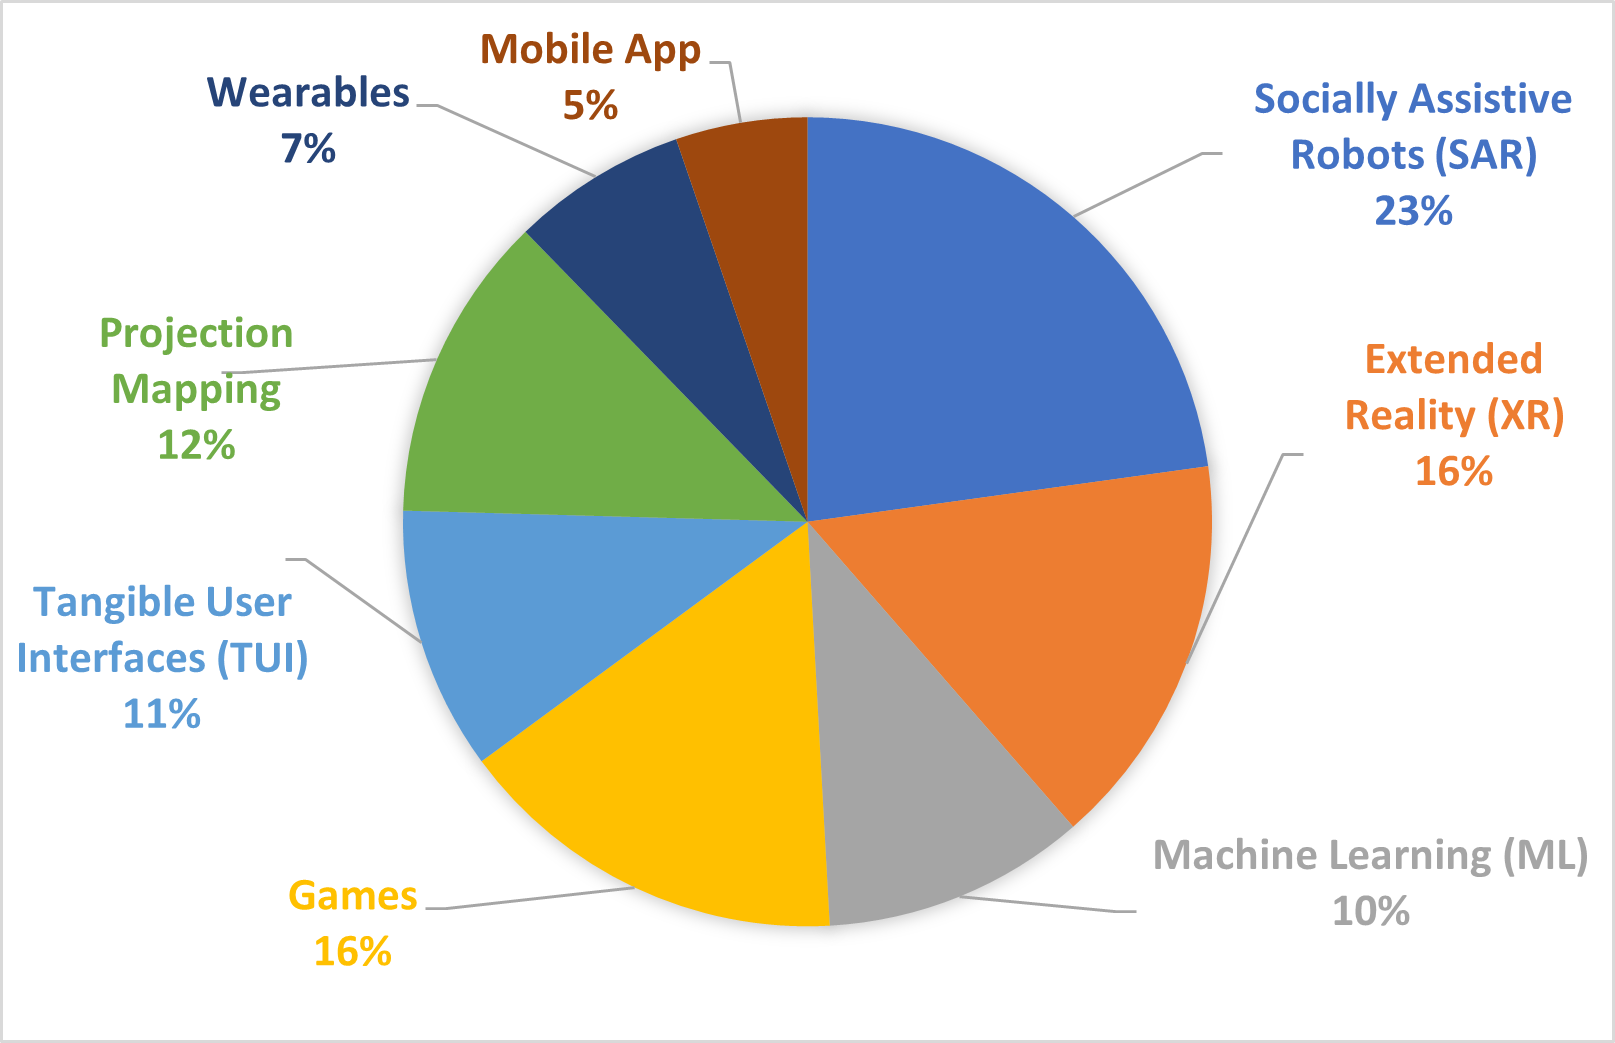
\includegraphics[width=0.65\textwidth]{fig6_tech-themes-general.png}
        \centering
	  \caption{Count of technology themes}\label{fig:tech-themes-count}
\end{figure}


In the observed years, we reflect the trend of these technologies, as seen on Figure \ref{fig:tech-themes-years}. SAR and video games are constantly evolving to provide interesting experiences, specially in children, therefore their relevance is kept during the years. XR and ML have gained popularity over the last years, with a contribution over the development of body trackers and immersive experiences. TUI and Wearables are relevant solutions in research for body movement, with a core on precision and data collection, though they have lost presence in recent works.

\begin{figure}
	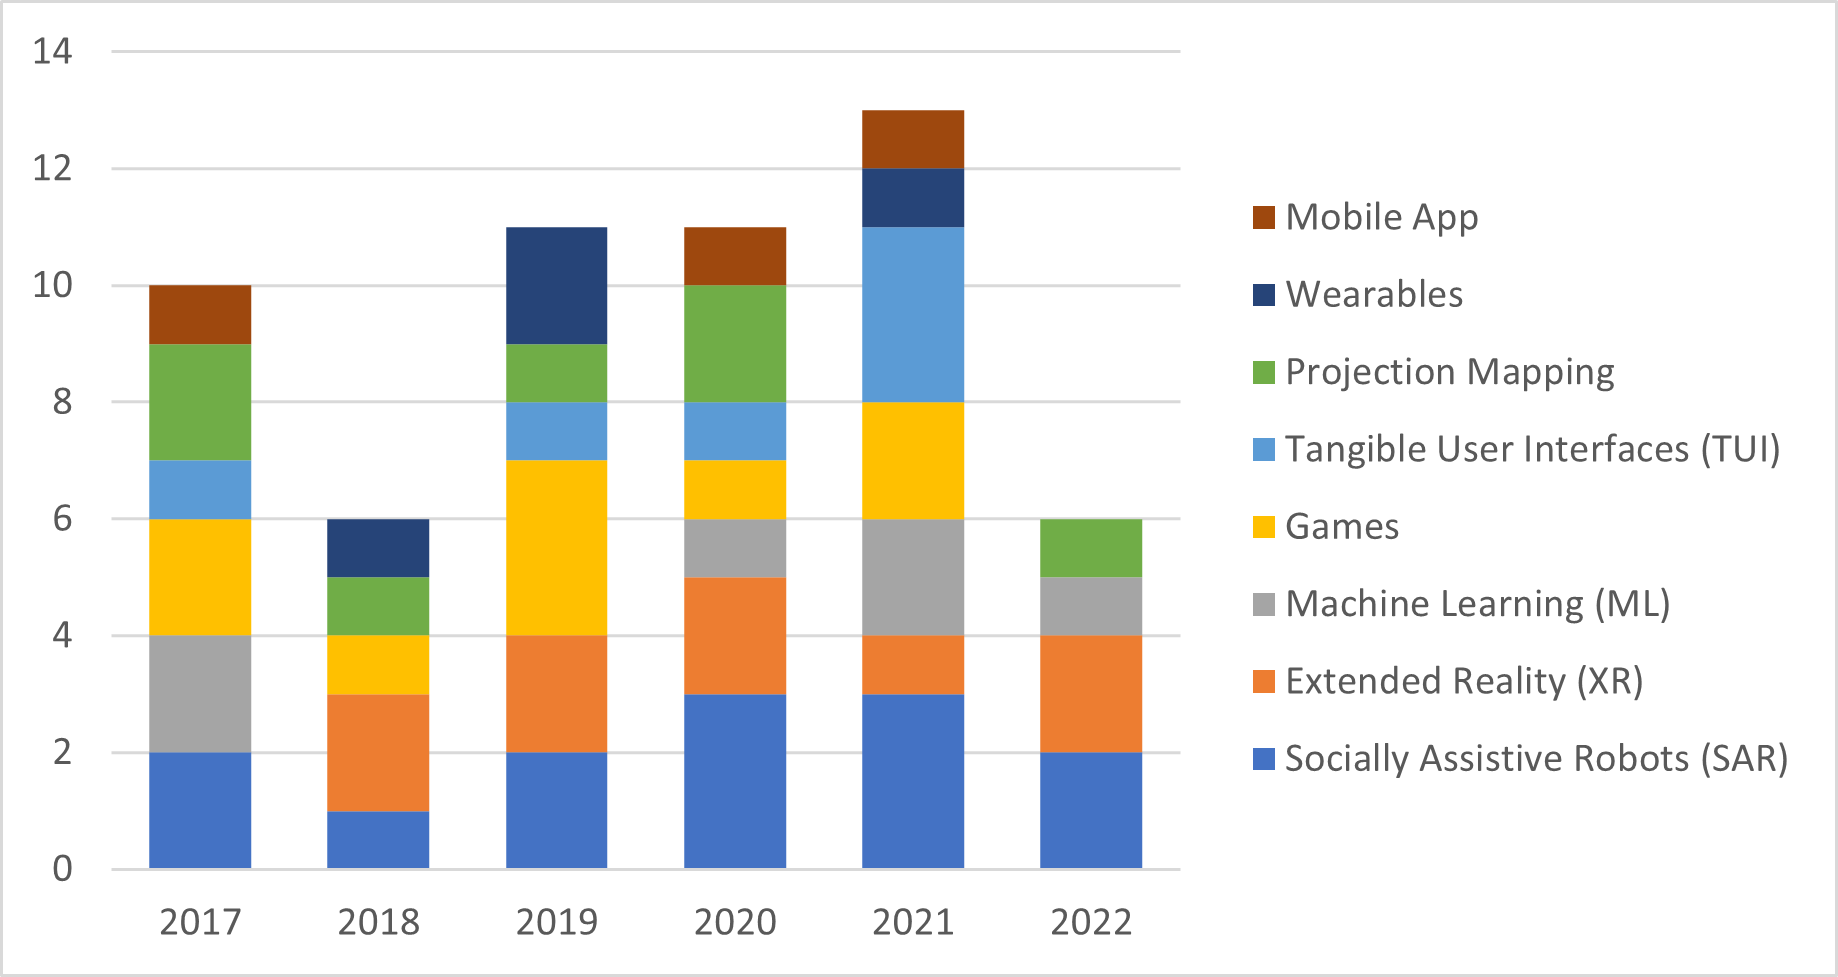
\includegraphics[width=0.65\textwidth]{fig7_tech-themes-years.png}
        \centering
	  \caption{Technology themes over the years}\label{fig:tech-themes-years}
\end{figure}


\hl{Body movement and recognition in the context of the DMT application are recognised through the utilisation of body trackers which capture the users' movements as the primary input. A body tracker functions as a mechanism that acquires data regarding the perceived position of the body, the movements of displayed limbs, the spatial distances involved, and the identification of typical movements and gestures. The prevalent types of body trackers include ML body figure models, various sensors, RGB-D technology, and video cameras. The analysis of recorded DMT sessions can involve either automated video analysis or manual examination conducted by proficient individuals. A general overview of the body tracking system for these studies is shown in Figure} \ref{fig:general-dmt-app} \hl{based on the pipeline for body recognition systems for HCI applications} \cite{Ahmed21}.

\begin{figure}
	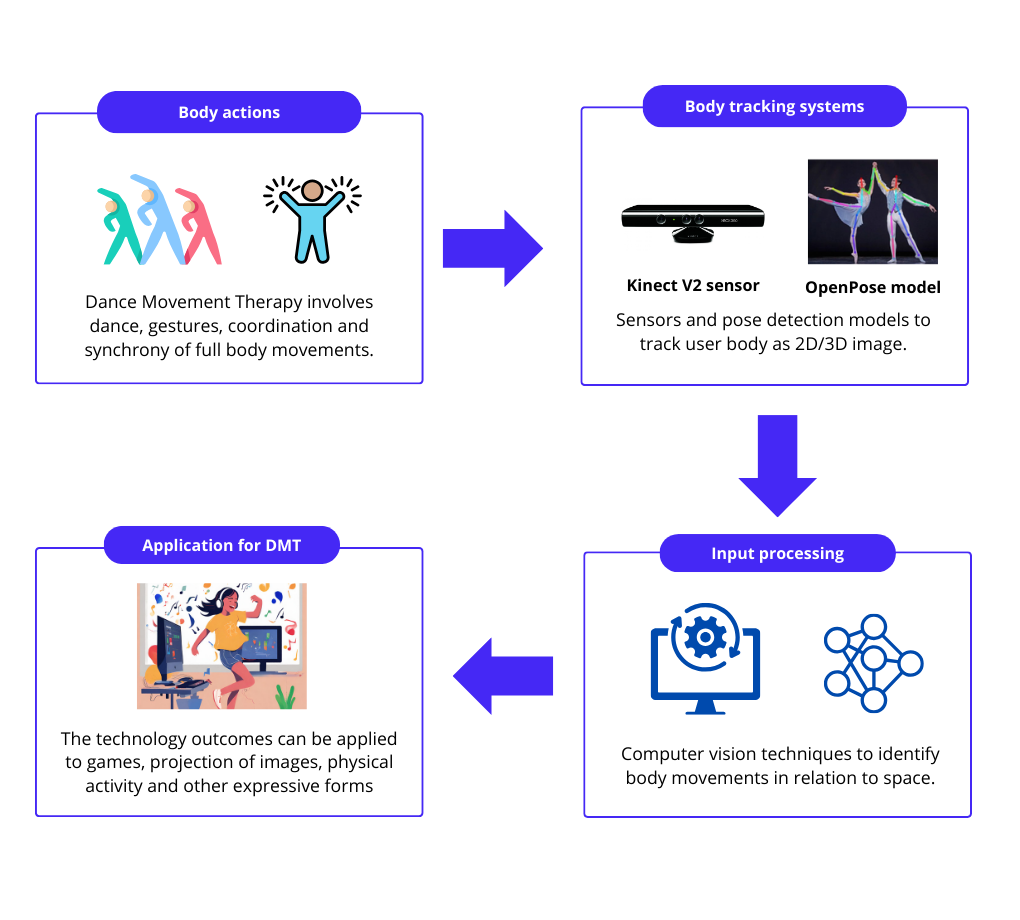
\includegraphics[width=0.9\textwidth]{fig-general-dmt-flow.png}
        \centering
	  \caption{\hl{General diagram for DMT applications with body trackers}}\label{fig:general-dmt-app}
\end{figure}

RGB-Depth cameras are used in a large group of studies, as they track body motions. In 22 studies, Microsoft Kinect is used to track the body of the user. 

This device consists of a depth camera that detects accurately the poses of the human body, with two versions (v1 and v2). Although it is the most predominant sensor used in research projects, current support is very limited. It has been discontinued for sale in 2017, Kinect originally has been designed for Xbox consoles with no computer extension, v2 is only compatible for Windows Software Development Kit (SDK). Contrasted with inertial measurement unit (IMU) sensors have reflected that Kinect gives sufficient data to perform free movement \cite{Geminiani19} 
Other similar cameras that have been used are AstraPro, Orbbec, Leap Motion, Xtion Asus/Openni2 \cite{Chevalier17} tracker sensors and Google Mediapipe \cite{DeCarolis21}.

Computer vision gives a preference for open-source models, the most popular is OpenPose. This Machine Learning model that represents the human body in 17 coordinate points. A total of 7 studies have used it, some combined with a Kinect to provide better accuracy. It is frequently updated, and the database is trained with user information. PoseNet is similar and used in one study \cite{Pohl20}.


\subsection{Expression and creativity}
\label{sec:4-express}
In certain projects, the interventions used dance as a creative and expressive form of therapy. Some included choreographic factors, music therapy and free movement expression. These studies are analysed to understand the outcomes of technology and main results for these applications, as it has been proven that DMT interventions have showed positive effects on body awareness, social competence, boundary perception of self and others well-being \cite{Koch23}. We reflect on the principal characteristics of these applications that focus on expression and creativity. We provide a summary of these works in table \ref{table:short-list} , that presents the selected interventions with the user group and DMT evaluation. Also, we have distinguished three groups for these applications according to purpose they follow.


\begin{table}[h]
\centering
\begin{tabular}{p{0.18\textwidth}|p{0.16\textwidth}|p{0.15\textwidth}|p{0.16\textwidth}|p{0.16\textwidth}}
\hline
\textbf{Application} & \textbf{Context}  & \textbf{Technology theme} & \textbf{DMT type} & \textbf{User evaluation} \\ [0.5ex] 
 \hline
Dance movement therapy with drones \cite{Ascensao22} & Dance Movement Therapy for coordination & Socially Assisted Robots & Dance, Imitation & 10 adults with ASD, aged 21-24 \\
\hline
Dance with NAO-robot \cite{Suzuki17} & Dance Movement Therapy & Socially Assisted Robots & Dance, imitation & 8 children with ASD, aged 4-10\\
\hline
Choreografish \cite{AltizerJr18} & Therapy, games & Virtual Reality & Coordination, rhythmic synchrony & 6 children with ASD \\
\hline
Motor proficiency with exercise game \cite{Hocking22} & Physical training, therapy & Virtual Reality & Coordination, imitation & 10 children with ASD aged 10-17\\
\hline
DanceCraft \cite{Ringland19} & Dance Movement Therapy & Projection Mapping & Dance, playful movements & 12 children with ASD aged 7-12 \\
\hline
GenPlay: Generative Landscape \cite{Crowell18} & Therapy, games & Projection Mapping & Dance, free movements, synchrony & 20 children with ASD aged 11-16\\
\hline
OSMoSIS \cite{Ragone20, Osmosis20}  & Music therapy  & Projection Mapping & Dance, synchrony & 11 children with ASD, aged 5-11\\
\hline
FroggyBobby \cite{Caro17}  & Exercise & Projection Mapping, Exergames & Coordination, body movement & 7 children with ASD aged 7-10 \\ 
\hline
Move \& Learn \cite{Raygoza-Romero21} & Therapy, games & Videogames & Visual-motor coordination, free movements & Children with NDD, validated with experts \\
\hline
ExpressiveBall \cite{Wilson20} & Playful games, expression skills development & Tangible User Interfaces &  Gestures, free body movement & 20 children with ASD, aged 4-8 \\
\hline
Motor imitation measurement \cite{Zampella21} & Imitation task, therapy & ML classification models & Coordination, imitation & 39 youth with ASD aged 9-17 \\
\hline
\end{tabular}
\caption{Summary of dance and expressive studies}
\label{table:short-list}
\end{table}

\subsubsection{Expression for social skills development} 

OSMoSIS (Observation of Social Motor Synchrony with an Interactive System) is a sound generation system with an embodied interface that converts movements into sounds, designed for music therapy sessions for children with ASD \cite{Ragone20, Osmosis20}. It promotes expression, communication, and social development, by a series of sounds inspired in the nature, children move their body in a free and expressive manner, captured by a Kinect. The video recordings of the sessions are transferred to the \hl{Motion Energy Analysis (MEA) software, presented as the most used tool to analyse interactions for ASD research} \cite{Ragone22}.

Children feel more engaged when they interact with the system, as they reflect better synchrony and social initiation with the facilitator of the therapy session. The system depicts a good example of DMT in a musical therapy context, where movements come along and motivate the final user to do the task and gain social strength.

GenPlay is a virtual environment system that transforms a standard classroom into an interactive play space \cite{Crowell18}. Children with ASD are interested in visual displays due to their high emotional response to their environment. This work seeks for collaboration between children in a projection of virtual objects based on generative graphics, projected in an interactive floor with a Kinect sensor.

Choreografish explores choreographic thinking in an activity to reduce anxiety in young adults with ASD \cite{AltizerJr18} and promote arts access. Participants control a virtual school of fish in a VR videogame based on the HTC Vive. This immersive environment helps soothe anxiety levels with the use of embodied choreographic thinking.

FroggyBobby is an exergame that supports eye-body coordination\cite{Caro17}. Children are instructed to move their arms to control a virtual frog that flies. After 7 weeks of sessions, children with severe autism proved to maintain their attention for the entire duration of therapy, reduced their aimless movement of the limb, and developed aimed movement of the limb.


\subsubsection{Dance for imitation and coordination}  %% 4.4.2
Therapy extends further to humans and now includes Socially Assistive Robots (SAR) to provide an adapted and responsive interaction. The next four interventions have robots as an interactive element during a dance movement therapy setup, where children imitate the robot movements or dance along with it.

The first project explores a new category for SAR, socially assistive drones (SAD), that are controlled by human movements \cite{Ascensao22}. It adapts a personalised interaction for DMT, implemented with a Parrot Bebop 2 drone powered by a control system and an image-processing-based data analysis module. Users control the drone based on fuzzy logic, which motivates the dance activities and engages their participation.

A different approach is to study a robot as an effective education agent for children with ASD during a DMT intervention for body recognition \cite{Suzuki17}. A small dance that identifies body parts with a song, head-shoulders-knees-clap, is explored with three instructors: a NAO robot, a therapist, and an unfamiliar person to the user. In this body identification task, robot-led therapy proved to be similar to human instructors, and, like the previous case, it is found to be more engaging and attractive for children during DMT.



\subsubsection{Dance in games and physical training}  %% 4.4.3

DanceCraft is a whole-body interface that augments dance movement therapy during home sessions \cite{Ringland19}. This game-like application uses recordings of dance instructors that are displayed on a screen, where users can play these dances and see a reflected image of their movements, as a ``skeleton'' in the same screen. It uses a camera, a Kinect sensor and has been developed with Processing, a framework for digital 3D graphics. A pilot study has been conducted with a group of children with ASD, that had dance movement therapy sessions in an institution with an instructor, and then a week of home sessions along with their families, resulting in an engaging and fun experience for them.

During motor imitation tasks, TD youth differentiates from ASD youth in terms of performance and biomarkers. A classification model proves there is no major difference between a 2D or 3D body joint tracking data \cite{Zampella21}. In this study, intra and interpersonal coordination features are classified with 82 \% accuracy.

Move \& Learn is an exergame that helps children with NDD with upper limb coordination exercises \cite{Raygoza-Romero21}, motor proficiency is also executed with an exercise game  \cite{Hocking22}.



% DISCUSSION
\section{Discussion} 
\label{sec5:discussion}
We have found a diversity of technological approaches that respond to our initial queries, ranging across different contexts and user groups, though few of them were applications directly related to dance and expression. DMT is a complex and evolving field, interventions as part of an art therapy process are valuable for individuals that need alternative forms of expression, but also feel represented as digital natives.

Human Computer Interaction (HCI) offers tools for these projects such as usability and accessibility guidelines, evaluation techniques and projection for improvements on the implementation, with a user centred design. There is plenty of room for research in the field, and some findings will be addressed as follows.

In Virtual scenarios, such as virtual characters displayed along the real environment. Virtual Reality (VR) takes an immersive approach, the users is embodied by a virtual character that moves in accordance with the users’ controllers. Augmented Reality (AR), on the other hand, takes a mobile device or glasses that mix both virtual and real objects. For a dance movement therapy, MR solutions are based on natural user movements for the embodied interface.

The three research questions are addressed in the following subsections.

\subsection{RQ1: \emph{What themes of application has technology contributed in DMT interventions for people diagnosed with ASD?}}

In subsection \ref{sec:app-contexts}, we have distinguished three major groups to classify DMT interventions with technology: therapy studies, including serious games, music and \hl{dance movement therapy}; physical training, including motor training systems and exercises, and general areas of behaviour and body expression.
In accordance to our research topic, the keyword ``therapy'' refers to various contexts of application for accessibility studies, whereas ``dance'' is associated with music and ``movement'' with motor skills, games and exercise.


Therapy with the use of games provides an engaging factor for children in the development of motor skills through gamification. Participants feel stimulated with these virtual activities, by the use of attracting visual graphics, characters and journeys based on storytelling to complete an action. Games are generally video based, use some form of Extended Reality and basic controllers. Other group are based on interactions with social robots.

Most interventions are made to improve motor skills like coordination, gesture control and imitation, guided by a virtual character or instructor. In this sense, the goal is to follow a set of movements or coordination activities, which are scored according to the performance of the result to an expected response. This limits the expressive aspect of the user as they depend on the scope of the game, generally to gain posture and physical movements control with a reduce on their stereotypical behaviour.

Music therapy in DMT is mainly focused on development of musical synchrony and coordination through body movements, following a pattern or tempo.
OSMoSIS \cite{Ragone20OS, Ragone22} is the only work that guides interaction into a musical expression form, where users receive interactive sound feedback according to their movements.  Music creation seen as an art therapy form should be taken into account, with the body as an interface to produce digital sounds. 

Only 4 works have been identified solely to use dance performance and non-structured body movements to guide the intervention. In the context of a DMT review, this number is little and represents that other interventions have an objective of motor skills development as a correction form to learn or adapt stereotypical behaviour and precise movements. People with ASD also need formation in creative and expressive skills, which can be developed with DMT, specially when in cases where norms and oral communication are still a challenge for them.

As part of the movement factor, other group of interventions relied on motor development as their focus of study. In general, works described in section \ref{sec:app-contexts-motor} classified as motor training and exercise were mostly based in mimics, balance, imitation and coordination tasks, with required hardware for detecting precise movements like sensors, cameras and wearables. Training systems in general are produced to achieve a better accuracy for users that struggle with body movement control. Complex hardware gives precision, though users with ASD need to reduce the devices they wear to reduce feeling overwhelmed, also simpler solutions are easier to understand and replicate, so alternatives to large installations with multiple devices must be found.

As for user participation, we note that children with ASD are the most frequent user group for evaluations.
Most studies are designed for children with ASD and other neurodevelopmental disorders, as therapy is recommended following their diagnosis in their early formation stages. Generally, they are the main participants, though some children prefer to participate accompanied by their caregivers or other children, in case they need to interact for social skills development.
Adults and elderly people with ASD may also benefit from these interventions, further research can provide space to design for adults with ASD.

The participation of therapists can be as a guide for intervention, in an active role like a virtual agent or instructor. Other cases include remote therapy with tele-rehabilitation mediated with a robot \cite{Rosly20}, observation with video analysis, and others were the therapist only provides the tools for app design. Future design can include actively therapists and caregivers, enable rich participation in the session which can help users to feel more comfortable and engaged to participate.

Interventions should include multidisciplinary profiles, specially from the creative industries such as artists, designers or musicians, that should work along therapists and psychologists to produce a richer experience. In general, studies were innovative in form but many failed to include variety in the type of dance and expressive factors. Users need to be encouraged to participate and the role of technologies should be part of the engagement factor, with new technological trends for the current digital society.


\subsection{RQ2: \emph{How is body movement instructed, captured and analysed in technological DMT applications for people diagnosed with ASD? }} 

In most applications, a body movement tracker is used, which consists on a device that replicated body coordinates. The most used is Microsoft’s Kinect, which gives a whole-body model.  It is currently and outdated device, as production stopped in 2019. Other market alternatives include  Kinect Azure is a framework for this, with a cloud support.

Alternatives exist and have been proven to be as effective for movement detections. RGB-D cameras provide enough data, compared to Inertial Measurement Units (IMU) and 3D depth, results are similar, in fact, Kinect-based setup was chosen as the best candidate for embodied mirroring in autism treatment \cite{Geminiani19}. We have seen that 2D and 3D cameras give similar precision results when tracking movement for youth with ASD \cite{Zampella21}, so it can be explored the use of simpler devices.

Through the universe of DMT applications, different body movements are instructed and captured in each study. The main groups of study are imitation, coordination, gestures and free movements. For each one, the strategy for data capture is approached differently.

Imitation tasks are mostly used for motor impairments development in therapeutic and training systems. NAO robots help children to feel associated to repeat movements by a human like form.  In SAR projects, robots come with integrated sensors and cameras. They are used to imitate the body movement and give better precision. Generally, children imitate movements given by robots for interactive games \cite{Geminiani19, Santos20, Santos21}, gesture control \cite{DeCarolis21} and interactive dance \cite{Ascensao22}.

During imitation tasks, the user has to follow an instructor or video avatar and the evaluation is how well the user replicates those tasks. In the studies for imitation of movements, an instructor gave the instructions and exercises that the users had to imitate. Some cases used a NAO robot \cite{Santos20}, virtual agent \cite{Giraud21}, video recording of therapist \cite{Li21}. Movement precision needs accurate precision. Studies were a comparison to an abstract ML model.

Video recording has been a preferred method for direct observation and body tracking. Cameras have a limited point of view, and this explains the use of RGB-D alternatives. Many studies combined the RGB-D camera like Kinect, to a Machine Learning Model. OpenPose has given nice results in terms of body segmentation and certainty points. It has other alternatives such as PoseNet, though it has improved in recent years.

Different approaches have been used for DMT interventions, each with a unique form of interaction and scope of study. Technological advances keep evolving and this is reflected on the selected groups. For instance, extended reality applications and virtual agents have increased over the last years, which gives possibilities that are richer to older projection mapping environments.

In a predominant therapeutic scenario, it is important to consider the real user needs and limitations. The sake to use complex and expensive hardware is not the most relevant aspect in the overall evaluation. Case studies were as simple as a personal computer connected to a video projector, and others were a more complex virtual reality exergame with body sensors. Overall, it has been proved that interventions don’t need to be as expensive, nor the technology must be the most advanced to reach better results. The purpose is to augment the dance and free movement experience with a simple user interface, that is as intuitive as possible. If many instructions and heavy documentation is necessary, we can get the opposite effect and limit the expressiveness.

When working with users with special needs, in this case, children diagnosed with ASD, the less the ornaments, the better. Wearables were used for movement detection, though some children feel their body movements are limited. Most solutions implied cameras and a body tracking system, which had almost the same effect on body precision measurement.

Socially Assistive Robots are the predominant approach for DMT interventions, particularly robots that are shaped as medium sized humanoids, programmed to play games with children. In human-robot interaction, partner robots make company of children, play and dance with them along they capture data of their interaction. It can be useful to simulate social and role play, but robots cannot replace interaction that comes with social play with other children. Some approaches tend to use a remote dynamic with a therapist that controls the robots, though is better when the experts are present in the overall interaction. Robots also are mostly used in imitation tasks; it is preferred to be used on instructions and body movement correction and not an expressive search.

It has been shown that children find robot-directed therapy more engaging, though it can be attractive with other technologies as well. In the analysed findings, children perform the activities well with a robot instructor, but still prefer a human therapist to guide the DMT process.


\subsection{RQ3: \emph{How are creativity and expression evaluated during technological DMT interventions for people diagnosed with ASD?}} 
We have reviewed applications for social integration, motor improvement and expression in section \ref{sec:4-express},  with a focus on the group of interventions that are directly related to dance and expression. This group represents less than a quarter of the selected studies, though they are analysed in more detail due to their importance of their evaluation aspects.

 Generally, these interventions are carefully designed to provide positive outcomes that are validated with results that aim for common difficulties in ASD. The evaluation in most cases in related to emotional and emotional responses, performance on motor skills, as well as the usability of the systems. In section \ref{sec:4-express} we grouped the studies in three categories depending on the main outcomes found.

Children were stimulated for social collaboration through joint coordination activities that used dance as a common factor for social play \cite{Raygoza-Romero21, Osmosis20, Zampella21} . The systems track the user closeness and interaction between peers for social initiation, which is evaluated over time to see results in previous phases and after several weeks of use of the applications \cite{Osmosis20}.


Imitation and coordination skills are evaluated by a comparison of expected body movements. The "skeleton" obtained by the tracking sensors locates the coordinates of the body key points that are analysed with pre-trained models. Generally, these interventions involve music or sounds to develop coordination by following a certain rhythm or tempo, which is common for music therapy studies.

Some studies aim to reduce stereotypical behaviour like hand flipped movements, although these should be validated and used as entry for motor creativity rather than pursuing and imitation or coordination aspect.
 
In Choreografish, choreographic thinking is explored for anxiety relief \cite{AltizerJr18}, evaluated with questionnaires for users before and after the interventions. GenPlay provides playful environment responses \cite{Crowell18} that give an entertainment factor. Children are keen to learn by playing with games, that helps them to develop creative skills.

%In general, studies prove that technology can be part of their treatment and has been widely validated. The role of the therapist can be remote, present, or a mix of both. As part of the lockdown, remote therapy has become more popular and more digital therapy applications must be developed.Many research papers are found in a preliminary stage, with only a pilot study. Few cases have a follow-up or bigger project behind.

\hl{Studies in general demonstrate that technology can play a significant role in the treatment process and has received extensive validation. The therapist's involvement can range from being remote, physically present, or a combination of both. Due to the lockdown measures, remote therapy has experienced a surge in popularity, leading to a growing need for the development of digital therapy applications. Numerous research articles are currently in the early stages, often limited to pilot studies, while only a small number of cases have subsequent follow-ups or are part of larger projects.}

\hl{In some recent works outside of this review, several promising technologies are being utilised to enhance social skills in individuals with autism through dance movement therapy. One such technology is the Robot‐Inspired Computer‐Assisted Adaptive Autism Therapy (RoboCA3T), which focuses on improving joint attention and imitation skills by integrating robot avatars and computer-assisted therapies within a web-based solution} \cite{Zahid24}\hl{. Additionally, the use of Mixed Reality Dance Movement Therapy (DMT) with interactive virtual agents has shown great potential in improving motor control abilities in children with ASD by offering immersive training content and multi-sensory feedback} \cite{Liu24}\hl{. These innovative approaches aim to maximise engagement, facilitate skill development, and provide a supportive environment for individuals with ASD to enhance their social communication, sensory sensitivities, and emotional regulation through tailored dance activities} \cite{Makheti24}.


% IMPLICATIONS FOR RESEARCH
\section{Implications for Research}
\label{sec6:implications}
In this section, we introduce the implications of this study, according to the main factors that have influenced the presented works and may be taken into account for future research, and the limitations of this study.

\subsection{General guidelines for future works}
Based on our revision, we include a set of guidelines that future research projects should follow for DMT applications. We identify the opportunities in the field, with the hope to find a more diverse set of applications in the future.

\subsubsection{Demography}

As part of the demographic factor, universal design has to consider all ages and contexts of users for a complete integration. Most projects focus on younger users, so there is a opportunity in design for adults and the elderly people with ASD. In the current literature, interventions serve for children to adapt and improve motor skills with technology applications, considering they have been raised in the 4.0 Industry world. They are digital natives, but many adults struggle with some advances and may need additional support to use these applications. Some challenges to address are the usability of the developed works to change aspects like font size, discoverability of the motor tasks and effective feedback.

Another aspect is to include other participants that are present in these interventions —caregivers and therapists. These roles are present in some studies, though they observe the process and sometimes interact with the participant with ASD, as they are the main communication partner. The idea is to provide a better design with the implication of these counterparts, that may help to view the effects on therapy from an external yet familiar point of view, to improve in more effective experiences. \hl{In general, psychotherapists agree that intervention plans should be designed for each patient, in accordance to their characteristics. In this sense, interventions are viewed as mini-games or activities that form part of their individual treatment and future work should provide a personalised follow up plan, with registration of qualitative information as notes or comments } \cite{Raygoza-Romero21}.

Design process in general should be user-oriented and complimented with the voice of professionals: experts in ASD, psychologists, artists, dancers and musicians and experts from related non-profit organisations. Interventions should enrich from interdisciplinary perspectives as these are made to change over time as part of a complementary therapy approach. \hl{It is key to provide a plan for flexible communication interaction for the therapist and the final user on each context, design should include all counterparts involved in the intervention} \cite{Castelhano17}. 

\subsubsection{Technology}

Integrating technology in Dance Movement Therapy (DMT) for autism spectrum disorder (ASD) offers several unique benefits. One major advantage is the enhancement of precision and personalization in therapeutic interventions. Technologies such as body trackers, augmented reality (AR), and socially assistive robots (SAR) enable therapists to tailor activities to the individual needs of each participant, which can significantly improve therapeutic outcomes. Additionally, technology can provide consistent feedback and support, which is particularly beneficial for individuals with ASD who may require more structured environments to thrive. Moreover, the use of interactive and engaging tools can increase motivation and participation, essential for the effectiveness of DMT. However, there are also drawbacks to consider. The complexity and intrusiveness of some technological devices can be overwhelming for individuals with ASD, potentially hindering rather than helping their engagement. Furthermore, the reliance on technology requires substantial initial investment and ongoing maintenance, which can be a barrier for many therapy centres \cite{Berenguer2020, Kouroupa2022}. It can be prone to malfunctions, such as software glitches or hardware failures, which can disrupt therapy sessions and reduce their effectiveness \cite{Boucenna2014}. There is a risk of becoming overly reliant on technology, which can lead to a less personalised and more mechanical therapeutic experience \cite{Maskey2014}.

In relation of current trends, Machine Learning is constantly evolving with fast and novel results. Pose and body detection models are more precise and portable than ever before, with models that have little statistical difference to results obtained by a Kinect or other RGB-D sensors. The input can either be a recorded video or a live performance, support for multiple users and correction for background is now available, but suitable conditions should be studied in order to provide a full augmentation.\hl{Additionally, there is a lack of post-secondary policies guiding the delivery of technology-aided instruction and intervention for autistic transition-age youth, highlighting the necessity for future policies to support the development, implementation, and evaluation of such interventions} \cite{Sherwood24}.

Devices should be portable, light-weight and affordable; in this context, less is more. People with ASD may be overwhelmed with the use of wearable devices that are too intrusive, complex user interfaces with excessive or poorly explained information. Simpler technologies are more engaging, overall user experience must be ahead of complex precision factors.
% \textit{Technology}
% \begin{itemize}
%     \item Adapt to current trends - ML provide growth opportunities for body and dance augmentation.
%     \item Add diversity on devices - use alternatives to Kinect and RGB-D sensors.
%     \item Promote low cost and portable installations - less is more, users with ASD prefer less complex apps and non-obtrusive sensors.
% \end{itemize}

\subsubsection{Intervention objectives}

So far, the interventions of the study have dealt with the improvement of motor, social and communication skills, as many other studies for ASD. Areas of creativity and self-expression are still in debt to be studied in more depth, likewise, logical thinking and verbal aspects can be learned though creative games. The goal is to pursue embodied interfaces through in future research — the embodied interface can be a canvas and the body a brush for expressing profound emotions.

Some common objectives of ASD research are emotion recognition and self-regulation, development of autonomy and social initiation. Future research has an open door for interaction aspects that are being studied by therapists, in order to contribute to other areas of research.

Nowadays, telehealth interventions have gained importance, specially after the global COVID-19 pandemic retained people at their homes. Therefore, tele-rehabilitation is yet to be explored in artistic endeavours, where the process can benefit from users that find their best comfort at their own home and personal spaces. Therapists are adapting to virtual and remote interventions, that require new applications for an effective development.  \hl{In the case of tele-rehabilitation and remote systems, technological research should extend to be used at home, adapted to physical space constraints and lighter systems to fit the family room. For the inclusion of users with motor disabilities, technology should extend for inclusive design that develops specific skills in tasks that are achievable and may progress during time} \cite{Vargas20}.

% \textit{Objective}
% \begin{itemize}
%     \item Focus on expression and creativity - go further in education for areas that have not been explored in depth.
%     \item Consider aspects of ASD improvement - such as emotion recognition, autonomy development.
%     \item Explore alternative forms of therapy - for instance, telerehabilitation and artistic explorations.
% \end{itemize}

\subsubsection{Content}

The content to be developed gets more powerful with creative coding, 3D graphics and new models. By exploring new alternative in the creation, like in extended reality applications, users get more motivated to participate in the DMT sessions and get better results. To do this, it is fundamental to apply creative coding, integrate with graphic libraries like Processing, A-Frame, Three.js and others. By extending, the parameters control of colours, shapes and figures the user feels engaged in a larger process.

Also, there is still room to explore techniques that can automatically assess incidences of synchrony and shape interactive patterns. Beyond the traditional art forms, embodied space is three-dimensional and can be complimented with parameters like time, speed and complexity of movements to create dynamic artistic pieces. Sensors can give precise confidence levels, but synchrony yet is hard to evaluate, more insights should be provided to achieve a better movement control.

Finally, as neurodevelopmental disorders are a lifetime condition, therapy interventions need to be designed for long-term impact. Some works consisted in short-term classes or workshops, that intend to be continued and improved in the near future \cite{Caro18, Krichmar2018, Vargas20, Ragone22}. This is partially explained as research projects depend on external funding and have defined finalisation dates. As a complementary therapy, the real impact of DMT interventions can be observed after several months of constant practice. This presents a challenge to motivate the user enough to prevent desertion, each intervention should be unique and engaging for the users.

% \textit{Content}
% \begin{itemize}
%     \item Creative coding as reference for works - benefit from new models, 3D graphics and visualisations.
%     \item  Explore techniques to automatically assess incidence of synchrony and shape interactive patterns
%     \item Design for long term - extend from workshops and classes, to provide a big impact in therapy for ASD.
% \end{itemize}


\subsection{Limitations for the review}
The reported bias for this study includes the availability of publications for the selected period, the information presented in the studies and the interpretation given by the authors. Overall, some considerations are given for future reproducibility of this study and to justify the information detailed in previous sections.

First, strict queries around the topics of \hl{dance movement therapy} in autism gives a few number of results as described in the previous sections, so the search had to be general in order to include all works. Generally, selected projects had relation to the topic, though discarded options had eye movement, motor rehabilitation, and medical aspects that used technology for medical purposes. \hl{The main bias for the selection proccess has been to decide in which sense these contributions fall under DMT or other related areas out of the scope of the study. The authors addressed this by performing the queries and listing the inclusion or exclusion criteria for each paper by separate, to decide altogether the final selection of studies to review.}

Second, some projects were distributed in multiple papers with different aspects. Papers with user evaluation and complete development are prioritised, though some unfinished works were included because of their relevant methodology and design. \hl{A grey area of themes has been approached, for instance, what is virtual and physical world, or what is considered therapy is present upon the author's assumptions, as technology oriented professionals.}

Third, categories were made to group different aspects. The diversity of the results had to be simplified in order to provide a quantification for the results overview. \hl{The heterogeneity of the revised studies has limited to give generalised outcomes, as each work included different user groups and scope of study.} 


%CONCLUSIONS
\section{Conclusions}
\label{sec6:conclusion}
We have conducted a systematic literature review to gather information \hl{on combining technology and Dance Movement Therapy (DMT) for people with an Autism Spectrum Disorder (ASD). Studies were classified based on technology, users, and objectives using the PRISMA guidelines. The review aimed to find DMT interventions for ASD with technological support from four databases and 57 selected papers, as part of the inclusion and exclusion criteria based on the PRISMA checklist} \cite{Pagen71}.

%With the PRISMA protocol we defined the inclusion and exclusion criteria, and the  research questions that shaped the literature review.
% %% 
% following research questions: 
% \begin{enumerate}
%     \item What themes of application has technology contributed in DMT interventions for people diagnosed with ASD?
%     \item How is body movement instructed, captured and analysed in technological DMT applications for people diagnosed with ASD?
%     \item How are creativity and expression evaluated during technological DMT interventions for people diagnosed with ASD?
% \end{enumerate}

%We aimed to gather studies that describe DMT interventions for people with ASD with a technological support. 
%The search was conducted in four databases: Scopus, ACM DL, WoS and IEEE Xplore. We selected the studies based on the inclusion and exclusion criteria defined based on the PRISMA checklist \cite{Pagen71}, with a final selection of 57 papers. We then collected the information from these studies and classified them depending on their topic and area.

\hl{The studies focused on technology areas such as Mixed Reality (MR), Projection Mapping and Socially Assistive Robots (SAR). These projects shared three major components: a body tracker, the tech interface and the DMT aspect to study}. These installations don't require expensive nor sophisticated hardware to provide good results, most cases were demos or projects that need a follow up.\hl{
These studies involved children with ASD, mostly aged between 5 and 12, in areas like therapy, games, and social behaviour. Guidelines were provided for future DMT intervention development based on the analysed information.}
%The areas of application involved therapy, games, educational activities, play and social behaviour. Generally, these studies involved children with ASD, in particular, those aged between 5 and 12.

% With the analysed information we provided guidelines on each application area as a consideration for future development of DMT interventions. 
Studies \hl{showed outcomes for social, communication and personality development skills, with few focusing on expressiveness. %This particular studies were more open and had a larger reception on the DMT behaviour for dance. 
Further research should explore how an embodied interface can integrate social and expressive aspects for tangible results.}

We \hl{provide general guidelines for future research, considering the results of the literature review. Future studies should involve a wider range of users, inclusive design for} therapists and caregivers, and collaboration with specialists from related disciplines like art and psychology.

%Technology should be portable and affordable, with an update in sensors and new Machine Learning trained models for pose detection. The outcome for these works should consider emotional recognition, creativity and self-expression to advance in aspects that have not been considered enough in recent research. Also, consider trends for remote \hl{dance movement therapy} interventions based on tele-rehabilitation. Future projects should enrich from current graphical possibilities to engage users, considering that these interventions are designed for long-term use in order to perceive positive outcomes.

\hl{Future technology should be portable, affordable, with updated sensors and Machine Learning models for pose detection. Emotional recognition, creativity, and self-expression should be considered for positive outcomes. Remote dance movement therapy interventions based on tele-rehabilitation should be explored. Projects should use current graphical possibilities to engage users for long-term positive outcomes.}

%With this overview, we plan to continue to work to improve DMT interventions. This review illustrates the common aspects that researchers should consider, although this area is open and has more space to explore. We encourage researchers to propose new forms of applications for expressive and social expressions.


\section*{Acknowledgements}
Removed for blind review

\subsection{Declaration of generative AI and AI-assisted technologies in the writing process}

During the preparation of this work the author(s) used Writefull in order to correct grammar and academic language check. After using this tool/service, the author(s) reviewed and edited the content as needed and take(s) full responsibility for the content of the publication.


\printcredits

%% Loading bibliography style file
%\bibliographystyle{model1-num-names}
\bibliographystyle{elsarticle-num}
%\bibliographystyle{cas-model2-names}

% Loading bibliography database
\bibliography{bibliography}

% Biography
\bio{}
% Here goes the biography details.
Biography removed for blind review
\endbio

\end{document}

